\chapter{實驗與效能評估}
\label{chapter:evaluation}

% https://hackmd.io/@calee/HkNQc2ByO/https%3A%2F%2Fhackmd.io%2FyR2SvjqNQayQeWL2onkvmg
% https://docs.google.com/spreadsheets/d/11vgvawzM0E8TF6rnjfOtI_Z4iHDMS9jvwvSfVkNA-jU

為驗證本論文設計之方法,將 free5GC 核心網路移植至 OpenNetVM,使用其所提供之 ABI 能有效提升核心網路之效能,本實驗分別對原生之 free5GC 核心網路部屬於 Ubuntu Linux,與經過 OpenNetVM 移植過後之 free5GC 核心網路一樣部屬於 Ubuntu Linux,分別對其控制端 (control plane) 與用戶端 (user plane) 之效能進行測試,最終比對其結果,以驗證經過 OpenNetVM 移植過後的 free5GC 核心網路確實能有效提供更好的性能。

\textbf{Baseline:} 實驗過程我們會分別對原生之 free5GC 與經過移植至 OpenNetVM 的 LH5GC 進行註冊流程、連線建立流程、與換手流程等三個流程作測試,並比較其控制層的效能分析,另外我們也會建立連線後的用戶端進行頻寬測試,最後我們也會比較基於 Berkeley Socket 與基於 OpenNetVM shared memory 的 SBI 的效能差別。

\section{實驗環境設定}
\label{sec:evaluation_env}

我們所使用的硬體與軟體規格如下表~\ref{tab:sys_env}。 \cnote{調 tab:sys\_env 位置}

% This LaTeX table template is generated by emacs 27.2
\begin{table}[htbp]
    \centering
    \begin{tabular}{|c|c|l|}
        \hline
        \textbf{節點} & \textbf{項目} & \multicolumn{1}{c|}{\textbf{規格、型號、說明}} \\
        \hline
        \multirow{6}{*}{Traffic} & CPU & Intel(R) Core(TM) i7-7700 CPU @ 3.60GHz \\
        \cline{2-3}
        & Core No. & 4 \\
        \cline{2-3}
        & NIC & Intel Corporation Ethernet Controller X710/X557-AT 10GBASE-T \\
        \cline{2-3}
        & OS & Ubuntu 18.04.5 LTS \\
        \cline{2-3}
        & Kernel & 5.4.0-60-generic \\
        \cline{2-3}
        & Software & MoonGen Packet Generator~\cite{github.MoonGen} \\
        \hline
        \multirow{8}{*}{CN} & CPU & Intel(R) Core(TM) i7-9700 CPU @ 3.00GHz \\
        \cline{2-3}
        & Core No. & 8 \\
        \cline{2-3}
        & NIC & Intel Corporation Ethernet Controller X710/X557-AT 10GBASE-T 1589 \\
        \cline{2-3}
        & OS & Ubuntu 20.04.1 LTS \\
        \cline{2-3}
        & Kernel & 5.4.0-65-generic \\
        \cline{2-3}
        & \multirow{3}{*}{Software} & free5GC v3.0.4 \\
        & & HL5GC \\
        & & RAN UE Simulator \\
        \hline
        \multirow{5}{*}{DN} & CPU & Intel(R) Core(TM) i5-4460  CPU @ 3.20GHz \\
        \cline{2-3}
        & Core No. & 4 \\
        \cline{2-3}
        & NIC & Intel Corporation Ethernet Controller 10G X550T \\
        \cline{2-3}
        & OS & Ubuntu 18.04.5 LTS \\
        \cline{2-3}
        & Kernel & 5.4.0-62-generic \\
        \hline
    \end{tabular}
    % [] 放的是顯示在 list of figure 的文字
    % {} 放的是顯示在圖下方的文字
    \caption[系統環境參數]{{\footnotesize 系統環境參數}}
    \label{tab:sys_env}
\end{table}

我們的實驗在邏輯上 (logically) 將系統分為三個部件,邊緣端 (edge)、核心網路 (core network)、與數據網路 (data network)。邊緣端在真實網路下即是手機、基地臺與相關部件,以下會以 UE-RAN simulator 代稱。核心網路如第二章節所講解的,是第五代行動通訊網路中,放在機房 (data center) 中,負責統籌處理控制端 (control plane) 與轉發 (forward)、封裝 (encapsulate)、解封裝 (decapsulate) 使用者端 (user plane)。而數據網路 (data network),則是泛指傳統網路 (Internet),即為大多數時候,手機使用者想要存取的服務之所在位置。

為了準確的區分流量產稱與流量轉送的中央處理器 (以下簡稱 CPU) 使用率,避免單一 CPU 需要同時產生流量與處理流量,我們的測試方法將流量產生器 (traffic generator)、核心網路、流量接收者 (traffic receiver) 分別部屬於不同的機器上,讓三者得以完全妥善使用三顆不同之 CPU。

因此在務實面 (physically) 上將系統切分成三個節點,分別模擬使用者端流量發送、基地臺與核網處理、資料網路回覆 (圖~\ref{fig:eva_node}),在節點與節點中我們都是使用 Intel 的 10Gbps 雙孔網卡與 CAT-6A RJ45 網路線連接。在 Node 1 上面我們使用 MoonGen~\cite{paper.MoonGen} 軟體來產生流量。在 Node 2 上面我們分別佈署原生的 free5GC v3.0.4 與修改過後的 LH5GC 作為核心網路測試,另外比較特別的是,我們也把自行開發的 RAN UE 模擬器佈署在 Node 2 上面而非 Node 1 上,此模擬器會模擬 5G SA 的控制訊號與核心網路建立連線。而在 Node 3 上主要模擬資料網路回復封包,但若是測試單純下行流量,則會在 Node 3 上啟動 MoonGen 來產生流量。

\pnote{改圖}
\begin{figure}[htbp]
    \centering
    \begin{tikzpicture}
        \tikzset{vertex/.style = {shape=rectangle,draw,minimum size=1.5em,align=center}}
        \tikzset{edge/.style = {<->,> = latex'}}
        % vertices
        \node[vertex] (a) at (10,) {Node 1\\Traffic Generator};
        \node[vertex] (b) at (15,) {Node 2\\Core Network};
        \node[vertex] (c) at (20,) {Node 3\\Data Network};
        %edges
        \draw[edge] (a) to (b);
        \draw[edge] (b) to (c);
    \end{tikzpicture}
    % [] 放的是顯示在 list of figure 的文字
    % {} 放的是顯示在圖下方的文字
    \caption[實驗環境節點]{{\footnotesize 實驗環境節點}}
    \label{fig:eva_node}
\end{figure}

\section{用戶層效能分析}
\label{sec:up_evaluation}

\subsection{上行流量分析}
\label{subsec:uplink_evaluation}

在用戶端的測試中,我們首先作了上行流量測試,分別使用不同大小的 ping 封包從 Node 1 藉由 Node 2 送至 Node 3,在這個測試中關閉 Node 3 回復 ping 的功能,觀察 Node 3 接收到的流量。

\subsection{來回流量比較}
\label{subsec:uldl_comp}

在這個測試中,我們比較 LH5GC 與 free5GC 上下行流量,除了關閉 Node 3 ping 回復功能的測項外,也測試了開啟回復功能後,Node 1 接收到的流量。

\begin{figure}[htb]
  \centering
  % 圖片的高度與寬度, height 設為 ! 代表由寬度大小等比例縮放
  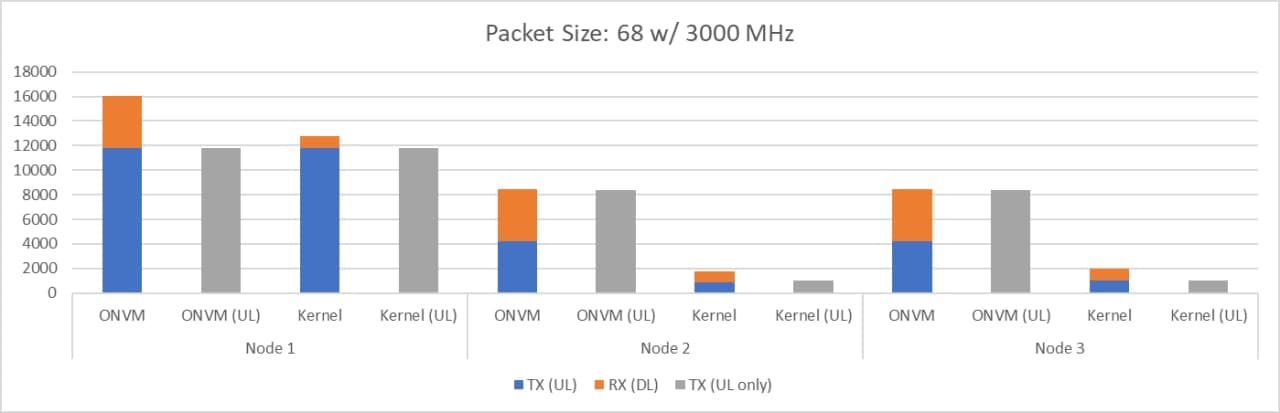
\includegraphics[height=!,width=1\linewidth,keepaspectratio=true]{figures/user_plan_performance}
  % [] 放的是顯示在 list of figure 的文字
  % {} 放的是顯示在圖下方的文字
  \caption[用戶層效能]{{\footnotesize 用戶層效能}}
  \label{fig:user_plan_performance}
\end{figure}

\subsection{CPU 時脈影響}
\label{subsec:cpu_clock}

由於在測試的過程中,我們發現 CPU 時脈會對劉量產稱可觀的影響,因此我們也嘗試測試 CPU 時脈與流量的關係。

\section{控制層效能分析}
\label{sec:cp_evaluation}

\subsection{PFCP 延遲差異}
\label{subsec:pfcp_comp}

\subsection{SBI 延遲差異}
\label{subsec:sbi_comp}

\subsection{控制流程延遲比較}
\label{subsec:cp_proc_comp}
